% !TEX root = ../main.tex
% File: chapters_part1/chap3_7.tex
% Nội dung cho Phần 3.7: Các Kiến trúc Nơ-ron Khác

\section{Các Kiến trúc Nơ-ron Khác}
\label{sec:other_nn_architectures}

Bên cạnh RNN, CNN và các kiến trúc chính khác, trong NLP còn tồn tại nhiều hướng tiếp cận nơ-ron đặc thù cho các dạng bài toán riêng. Phần này sẽ trình bày hai kiến trúc tiêu biểu: \textbf{Mạng Siamese} cho việc học sự tương đồng, và \textbf{Mạng Nơ-ron Đồ thị (GNNs)} cho việc xử lý dữ liệu có cấu trúc đồ thị.

\subsection{Mạng Siamese (Siamese Networks) cho việc học sự tương đồng}
\label{ssec:siamese_networks}

Các kiến trúc chúng ta đã học như RNN hay CNN thường được huấn luyện cho các tác vụ phân loại (classification) hoặc gán nhãn (labeling). Tuy nhiên, có một lớp bài toán rất quan trọng trong NLP mà các kiến trúc này không trực tiếp giải quyết được: \textbf{đo lường sự tương đồng ngữ nghĩa (semantic similarity)} giữa hai câu. Ví dụ:
\begin{itemize}
    \item \textbf{Phát hiện câu hỏi trùng lặp (Duplicate Question Detection):} Trên các diễn đàn như Quora hay Stack Overflow, việc xác định xem một câu hỏi mới có trùng lặp về mặt ý nghĩa với một câu hỏi đã có hay không là rất quan trọng.
    \item \textbf{Tìm kiếm ngữ nghĩa (Semantic Search):} Tìm các tài liệu có ý nghĩa liên quan nhất đến một câu truy vấn, thay vì chỉ khớp từ khóa.
    \item \textbf{Đánh giá câu trả lời của sinh viên (Automatic Short Answer Grading):} So sánh câu trả lời của sinh viên với câu trả lời mẫu để chấm điểm.
\end{itemize}

Để giải quyết các bài toán này, chúng ta cần một mô hình có khả năng nhận vào hai câu và xuất ra một điểm số thể hiện mức độ tương đồng của chúng. Mạng Siamese \cite{mueller2016siamese} là một kiến trúc thanh lịch và mạnh mẽ được thiết kế cho chính mục đích này.

\subsubsection{Tư duy cốt lõi: Học một không gian biểu diễn tốt}
\label{ssec:siamese_intuition}

Thay vì cố gắng học một hàm phân loại trực tiếp trên cặp câu, ý tưởng cốt lõi của Mạng Siamese là \textbf{học một hàm nhúng (embedding function) có khả năng ánh xạ các câu vào một không gian vector (embedding space) sao cho trong không gian đó, khoảng cách giữa các câu có thể phản ánh sự tương đồng về mặt ngữ nghĩa của chúng}.

Nói một cách cụ thể hơn, Mạng Siamese học cách để:
\begin{itemize}
    \item Các cặp câu \textbf{tương tự} (similar pairs) được kéo lại \textbf{gần nhau} trong không gian embedding.
    \item Các cặp câu \textbf{không tương tự} (dissimilar pairs) bị đẩy ra \textbf{xa nhau} trong không gian embedding.
\end{itemize}

Sau khi đã học được không gian embedding tốt này, việc đo độ tương đồng giữa hai câu mới chỉ đơn giản là ánh xạ chúng vào không gian này và tính khoảng cách Euclide hoặc độ tương đồng cosine giữa hai vector kết quả.

\subsubsection{Kiến trúc Mạng Siamese}
\label{ssec:siamese_architecture}

Cái tên "Siamese" (cặp song sinh dính liền) mô tả rất chính xác kiến trúc của nó. Mạng Siamese bao gồm hai "nhánh" (towers) mạng nơ-ron giống hệt nhau, xử lý hai đầu vào một cách song song.

\paragraph{Hai nhánh, một bộ não}
\begin{itemize}
    \item Mạng bao gồm hai bộ mã hóa (encoder) có \textbf{kiến trúc y hệt nhau}.
    \item Quan trọng nhất, hai bộ mã hóa này \textbf{chia sẻ cùng một bộ trọng số (share weights)}. Điều này có nghĩa là chúng ta chỉ có một "bộ não" duy nhất, được áp dụng cho cả hai câu đầu vào.
    \item Việc chia sẻ trọng số đảm bảo rằng hai câu giống hệt nhau sẽ luôn được ánh xạ tới cùng một điểm trong không gian embedding. Nó cũng làm cho mô hình hiệu quả hơn nhiều về mặt tham số.
    \item Bộ mã hóa này có thể là bất kỳ kiến trúc nào có khả năng biến một chuỗi thành một vector, ví dụ như một mạng LSTM, GRU, hoặc CNN đã được học ở các phần trước.
\end{itemize}

\begin{center}
    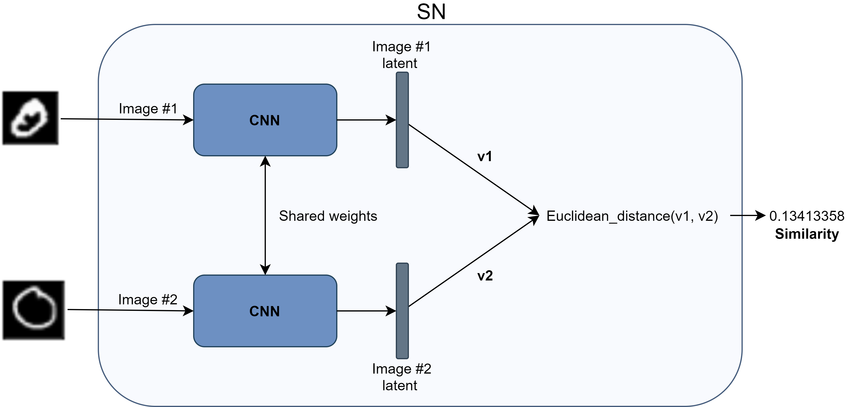
\includegraphics[width=0.7\textwidth]{siamese_network_architecture.png}
    \captionof{figure}{Kiến trúc của Mạng Siamese. Hai mạng con (thường là LSTM hoặc CNN) có cùng kiến trúc và chia sẻ trọng số. Chúng xử lý hai câu đầu vào để tạo ra hai vector embedding. Hàm mất mát sau đó được tính toán dựa trên khoảng cách giữa hai vector này.}
    \label{fig:siamese_network_architecture}
\end{center}

\subsubsection{Hàm Mất mát Tương phản (Contrastive Loss)}
\label{ssec:contrastive_loss}
Kiến trúc chỉ là một nửa câu chuyện. Phép màu thực sự của Mạng Siamese nằm ở hàm mất mát đặc biệt được sử dụng để huấn luyện nó: \textbf{Hàm Mất mát Tương phản (Contrastive Loss) \cite{hadsell2006dimensionality}}.

Hàm mất mát này được thiết kế để thực hiện chính xác mục tiêu mà chúng ta đã đề ra: kéo các cặp tương tự lại gần và đẩy các cặp không tương tự ra xa.

\paragraph{Đầu vào huấn luyện}
Để huấn luyện với Contrastive Loss, chúng ta cần một bộ dữ liệu bao gồm các bộ ba: (\texttt{câu\_A}, \texttt{câu\_B}, nhãn).
\begin{itemize}
    \item \textbf{Nhãn $Y=1$ (Cặp Tương tự):} \texttt{câu\_A} và \texttt{câu\_B} có cùng ý nghĩa.
    \item \textbf{Nhãn $Y=0$ (Cặp Không Tương tự):} \texttt{câu\_A} và \texttt{câu\_B} có ý nghĩa khác nhau.
\end{itemize}


\paragraph{Công thức}
Cho một cặp đầu vào, Mạng Siamese tạo ra một cặp vector embedding $(v_A, v_B)$. Chúng ta định nghĩa $D_W$ là khoảng cách Euclide giữa chúng: $D_W = ||v_A - v_B||_2$.

Hàm mất mát tương phản được định nghĩa như sau:
\begin{equation}
    \text{Loss}(W, (Y, v_A, v_B)) = Y \cdot \frac{1}{2} D_W^2 + (1-Y) \cdot \frac{1}{2} \max(0, m - D_W)^2
    \label{eq:contrastive_loss}
\end{equation}
Trong đó $m$ là một siêu tham số gọi là \textbf{lề (margin)}.

\paragraph{Phân tích hàm mất mát}
Hãy xem hàm mất mát này hoạt động như thế nào trong hai trường hợp:
\begin{enumerate}
    \item \textbf{Khi cặp câu là Tương tự ($Y=1$):}
        \begin{itemize}
            \item Phần thứ hai của công thức bị triệt tiêu (vì $1-Y=0$).
            \item Hàm mất mát trở thành: $\text{Loss} = \frac{1}{2} D_W^2$.
            \item Để tối thiểu hóa loss, mô hình phải làm cho khoảng cách $D_W$ càng gần 0 càng tốt. Điều này \textbf{kéo hai vector lại gần nhau}.
        \end{itemize}
    \item \textbf{Khi cặp câu là Không Tương tự ($Y=0$):}
        \begin{itemize}
            \item Phần đầu của công thức bị triệt tiêu (vì $Y=0$).
            \item Hàm mất mát trở thành: $\text{Loss} = \frac{1}{2} \max(0, m - D_W)^2$.
            \item Để tối thiểu hóa loss, mô hình phải làm cho $m - D_W$ nhỏ hơn hoặc bằng 0, tức là $D_W \geq m$.
            \item Điều này \textbf{đẩy hai vector ra xa nhau} cho đến khi khoảng cách giữa chúng ít nhất là bằng lề $m$. Nếu chúng đã đủ xa ($D_W > m$), loss sẽ bằng 0 và mô hình không cần phải làm gì thêm.
        \end{itemize}
\end{enumerate}
Lề $m$ đóng vai trò như một "vùng an toàn", nó yêu cầu các cặp không tương tự phải cách nhau một khoảng tối thiểu, tạo ra sự phân tách rõ ràng trong không gian embedding.

\subsubsection{Triplet Loss: Một sự thay thế nâng cao}
\label{ssec:triplet_loss}

Một hàm mất mát phổ biến khác, có liên quan chặt chẽ, là \textbf{Triplet Loss \cite{schroff2015facenet}}. Thay vì huấn luyện trên các cặp, Triplet Loss huấn luyện trên các bộ ba (triplets) gồm:
\begin{itemize}
    \item \textbf{Anchor (A):} Một câu neo.
    \item \textbf{Positive (P):} Một câu tương tự với Anchor.
    \item \textbf{Negative (N):} Một câu không tương tự với Anchor.
\end{itemize}

Mục tiêu của Triplet Loss là làm cho khoảng cách từ Anchor đến Positive nhỏ hơn khoảng cách từ Anchor đến Negative, cộng với một lề $m$.
$$ d(A, P) + m < d(A, N) $$
Hàm mất mát được định nghĩa là:
\begin{equation}
    \text{Loss} = \max(0, d(A, P) - d(A, N) + m)
    \label{eq:triplet_loss}
\end{equation}
Triplet Loss thường được coi là mạnh mẽ hơn vì nó trực tiếp tối ưu hóa thứ hạng tương đối giữa các câu, thay vì chỉ xem xét các cặp một cách riêng lẻ. Tuy nhiên, việc tạo ra các bộ ba huấn luyện hiệu quả (hard triplets) là một thách thức kỹ thuật.

\subsubsection{Tổng kết}
Mạng Siamese và các hàm mất mát đi kèm (Contrastive/Triplet Loss) là một bộ công cụ cực kỳ mạnh mẽ cho các bài toán so sánh. Chúng không chỉ giới hạn trong NLP mà còn được áp dụng rộng rãi trong xử lý ảnh để nhận dạng khuôn mặt (face verification) hay tìm kiếm ảnh tương tự.

Thay vì học cách phân loại, Mạng Siamese học cách \textbf{biểu diễn}, tạo ra các embedding chất lượng cao, có thể tái sử dụng cho nhiều tác vụ hạ nguồn liên quan đến đo lường sự tương đồng.

\subsection{Mạng Nơ-ron Đồ thị (Graph Neural Networks - GNNs) trong NLP}
\label{ssec:gnn_for_nlp}

Trong suốt chương này, chúng ta đã xem xét các kiến trúc được thiết kế để xử lý dữ liệu dạng \textbf{chuỗi (sequences)} như RNN và các kiến trúc trích xuất đặc trưng cục bộ như CNN. Tuy nhiên, một sự thật quan trọng là: \textbf{ngôn ngữ không phải lúc nào cũng là một chuỗi tuyến tính}. Rất nhiều thông tin quý giá trong ngôn ngữ và thế giới mà nó mô tả lại có cấu trúc của một \textbf{đồ thị (graph)}.

Ví dụ:
\begin{itemize}
    \item Cấu trúc cú pháp của một câu (như Cú pháp Phụ thuộc đã học ở Chương 1) là một đồ thị.
    \item Một cơ sở tri thức (Knowledge Base) về các thực thể và mối quan hệ của chúng là một đồ thị.
    \item Một mạng xã hội, với người dùng và mối quan hệ bạn bè, là một đồ thị.
    \item Một cuộc hội thoại nhiều bên, với các lượt lời và quan hệ trả lời, là một đồ thị.
\end{itemize}

Các kiến trúc truyền thống như RNN và CNN gặp khó khăn trong việc mô hình hóa các mối quan hệ phức tạp, không tuần tự này. Mạng Nơ-ron Đồ thị (GNNs) \cite{scarselli2009graph, kipf2016semi} ra đời như một giải pháp tổng quát và mạnh mẽ để học trực tiếp trên dữ liệu có cấu trúc đồ thị.

\subsubsection{Nguyên lý Cốt lõi của GNN: Lan truyền Thông điệp (Message Passing)}
\label{ssec:gnn_message_passing}

Để hiểu GNN, trước hết ta cần hiểu cách nó "suy nghĩ" về một đồ thị. Một đồ thị bao gồm các \textbf{nút (nodes)} và các \textbf{cạnh (edges)} nối giữa chúng. Trong GNN, mỗi nút có một vector đặc trưng (node feature vector) riêng. Mục tiêu của GNN là học một hàm để tính toán một \textbf{vector biểu diễn (node representation/embedding)} cho mỗi nút, sao cho vector này không chỉ chứa thông tin của chính nút đó mà còn tóm tắt được thông tin từ \textbf{cấu trúc lân cận} của nó.

GNN thực hiện điều này thông qua một quy trình lặp đi lặp lại gọi là \textbf{Lan truyền Thông điệp (Message Passing)} hoặc \textbf{Tổng hợp Lân cận (Neighborhood Aggregation)}.

\begin{tcolorbox}[
    title=Trực giác về Lan truyền Thông điệp,
    colback=green!5!white, colframe=green!60!black, fonttitle=\bfseries
]
Hãy tưởng tượng mỗi nút trong đồ thị là một người. Tại mỗi vòng, mỗi người sẽ làm hai việc:
\begin{enumerate}
    \item \textbf{Gửi thư:} Gửi một bản sao "trạng thái" hiện tại của mình cho tất cả những người hàng xóm.
    \item \textbf{Cập nhật bản thân:} Nhận tất cả "thư" từ hàng xóm, tổng hợp chúng lại thành một thông điệp duy nhất, và sau đó kết hợp thông điệp này với trạng thái cũ của mình để tạo ra một trạng thái mới, thông thái hơn.
\end{enumerate}
Khi quá trình này lặp lại nhiều lần, thông tin từ những nút ở xa sẽ dần dần lan truyền khắp đồ thị. Một nút sau $k$ vòng lặp sẽ có một vector biểu diễn chứa thông tin từ tất cả các nút cách nó $k$ bước chân.
\end{tcolorbox}

Về mặt kỹ thuật, một lớp GNN thực hiện 3 bước:
\begin{enumerate}
    \item \textbf{Thu thập (Gather):} Với mỗi nút, thu thập vector đặc trưng từ tất cả các nút hàng xóm trực tiếp của nó.
    \item \textbf{Tổng hợp (Aggregate):} Áp dụng một hàm tổng hợp (ví dụ: `SUM`, `MEAN`, `MAX`) lên các vector đã thu thập để tạo ra một "thông điệp" lân cận duy nhất. Hàm này phải không nhạy cảm với thứ tự của các hàng xóm.
    \item \textbf{Cập nhật (Update):} Kết hợp thông điệp lân cận với vector đặc trưng hiện tại của nút (thường thông qua một mạng nơ-ron nhỏ) để tạo ra vector đặc trưng mới cho nút đó ở lớp tiếp theo.
\end{enumerate}

\begin{center}
    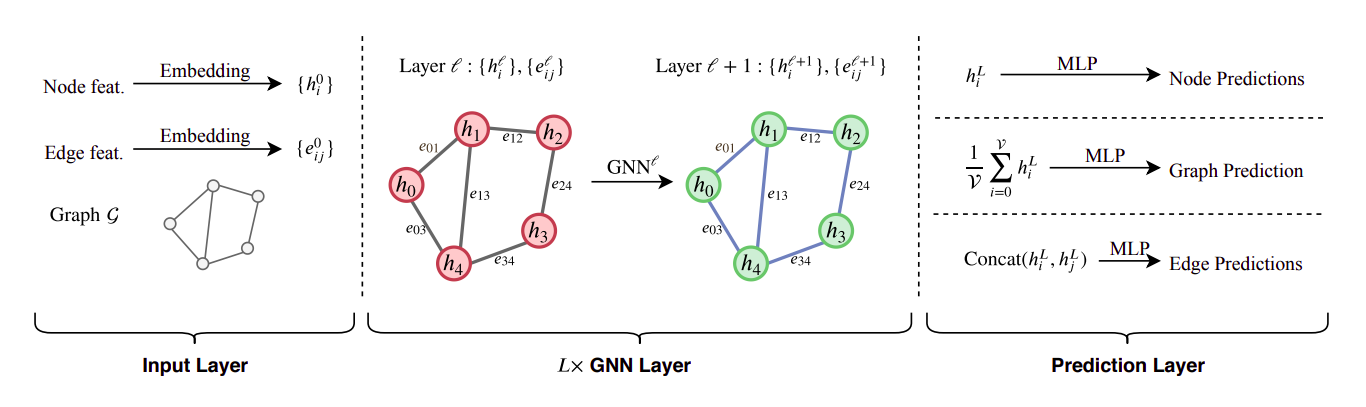
\includegraphics[width=1.0\textwidth]{gnn_message_passing.png}
    \captionof{figure}{Quy trình Lan truyền Thông điệp trong một lớp GNN. Nút A cập nhật trạng thái của nó bằng cách tổng hợp thông tin từ các hàng xóm B, C, D.}
    \label{fig:gnn_message_passing}
\end{center}

Bằng cách xếp chồng nhiều lớp GNN, một nút có thể tích hợp thông tin từ các hàng xóm ngày càng xa, cho phép mô hình có được "cái nhìn toàn cảnh" về vị trí và vai trò của mỗi nút trong toàn bộ đồ thị.

\subsubsection{Huấn luyện GNN}
Quá trình huấn luyện một GNN phụ thuộc vào tác vụ cụ thể ở cấp độ đồ thị, nút, hoặc cạnh.
\begin{itemize}
    \item \textbf{Tạo biểu diễn nút:} Sau $k$ lớp Message Passing, mỗi nút sẽ có một vector biểu diễn cuối cùng $h_v^{(k)}$ chứa thông tin từ lân cận $k$-bước của nó.
    \item \textbf{Hàm Mất mát:} Vector biểu diễn này sau đó được đưa vào một lớp đầu ra (ví dụ, một lớp FNN) để thực hiện dự đoán.
        \begin{itemize}
            \item \textbf{Phân loại Nút:} Lỗi (ví dụ, Cross-Entropy) được tính toán cho từng nút và lan truyền ngược qua các lớp GNN để cập nhật các trọng số của hàm tổng hợp (Aggregate) và cập nhật (Update).
            \item \textbf{Phân loại Đồ thị:} Các biểu diễn của tất cả các nút trong đồ thị được tổng hợp lại (ví dụ, qua pooling) thành một vector biểu diễn đồ thị duy nhất trước khi đưa vào lớp phân loại.
        \end{itemize}
\end{itemize}
Tương tự như các mạng khác, toàn bộ quá trình được tối ưu hóa end-to-end thông qua backpropagation.

\subsubsection{Các Ứng dụng then chốt của GNN trong NLP}
\label{ssec:gnn_applications}

Với khả năng học trên cấu trúc, GNN mở ra nhiều hướng ứng dụng mạnh mẽ trong NLP.

\paragraph{Làm việc với Đồ thị Tri thức và Mạng xã hội}
Đây là ứng dụng tự nhiên nhất của GNN. Trong một \textbf{Đồ thị Tri thức (Knowledge Graph - KG)}, các nút là các thực thể (ví dụ: `Hà Nội`, `Việt Nam`) và các cạnh có nhãn là các mối quan hệ (ví dụ: `isCapitalOf`).
GNN được sử dụng để giải quyết hai bài toán chính:
\begin{itemize}
    \item \textbf{Phân loại Nút (Node Classification):} Dự đoán một thuộc tính còn thiếu của một thực thể. Ví dụ, dự đoán thể loại của một bộ phim dựa trên các diễn viên và đạo diễn (các nút lân cận) của nó.
    \item \textbf{Dự đoán Liên kết (Link Prediction):} Đây là bài toán \textbf{trích xuất quan hệ và suy luận logic}. Mô hình dự đoán xem liệu một cạnh (mối quan hệ) có nên tồn tại giữa hai nút hay không. Ví dụ, nếu KG có các cạnh `(David Beckham, playsFor, Manchester United)` và `(Manchester United, locatedIn, England)`, GNN có thể học cách suy luận ra một liên kết tiềm năng `(David Beckham, hasNationality, English)`. Điều này cho phép tự động hoàn thiện và mở rộng các KG.
\end{itemize}

\paragraph{Phân tích Cú pháp dựa trên Đồ thị (Graph-based Parsing)}
Như đã đề cập, cây cú pháp phụ thuộc của một câu là một đồ thị. Chúng ta có thể áp dụng GNN trực tiếp lên cấu trúc này.
\begin{itemize}
    \item \textbf{Biểu diễn ngữ nghĩa dựa trên cấu trúc (Structure-aware Semantic Representation):} Thay vì chỉ dựa vào thứ tự tuần tự như LSTM, GNN cho phép một từ được biểu diễn bởi một vector tổng hợp thông tin từ các từ "quản lý" và "phụ thuộc" của nó. Ví dụ, vector của một động từ sẽ được "làm giàu" bởi thông tin từ chủ ngữ và tân ngữ của nó. Các biểu diễn này thường nắm bắt ngữ nghĩa chức năng tốt hơn.
    \item \textbf{Cải thiện các tác vụ hạ nguồn:} Các biểu diễn giàu cú pháp này sau đó có thể được sử dụng để cải thiện hiệu năng của các tác vụ như Trích xuất Quan hệ hay Phân tích Cảm xúc.
\end{itemize}

\paragraph{Mô hình hóa Hội thoại (Dialogue Modeling)}
Một cuộc hội thoại, đặc biệt là với nhiều người tham gia, không phải là một chuỗi tuyến tính.
\begin{itemize}
    \item \textbf{Xây dựng Đồ thị Hội thoại (Dialogue Graph):} Chúng ta có thể xây dựng một đồ thị trong đó các nút là các lượt lời (utterances), và các cạnh biểu diễn các mối quan hệ như "ai trả lời ai" hoặc "các lượt lời của cùng một người".
    \item \textbf{Ứng dụng GNN:} GNN có thể được chạy trên đồ thị này để học biểu diễn cho mỗi lượt lời, có tính đến toàn bộ lịch sử tương tác. Điều này rất hữu ích cho các tác vụ như tóm tắt hội thoại, theo dõi trạng thái hội thoại (dialogue state tracking), hoặc xác định cảm xúc trong các cuộc trò chuyện phức tạp.
\end{itemize}

\subsubsection{Các Kiến trúc Lai ghép: Kết hợp GNN và Transformer}
\label{ssec:gnn_transformer}

Sự ra đời của Transformer (sẽ học ở chương sau) đã thống trị NLP với khả năng nắm bắt phụ thuộc tầm xa trong chuỗi. Tuy nhiên, Transformer vốn không được thiết kế để xử lý thông tin cấu trúc tường minh. Điều này đã dẫn đến một hướng nghiên cứu sôi nổi: \textbf{kết hợp GNN và Transformer}.
\begin{itemize}
    \item \textbf{Ý tưởng:} Sử dụng Transformer để có được các biểu diễn từ ban đầu, giàu ngữ cảnh tuần tự. Sau đó, xây dựng một đồ thị (ví dụ: đồ thị cú pháp) lên trên các từ này và sử dụng GNN để "tinh chỉnh" (refine) các biểu diễn đó bằng cách cho chúng lan truyền thông tin qua cấu trúc đồ thị.
    \item \textbf{Kết quả:} Các mô hình lai ghép này thường cho kết quả tốt hơn trên các tác vụ đòi hỏi cả sự hiểu biết về cấu trúc và ngữ cảnh, ví dụ như các bài toán suy luận phức tạp.
\end{itemize}

\subsubsection{Thách thức và Hướng nghiên cứu Tương lai}
\label{ssec:gnn_challenges}
Mặc dù rất mạnh mẽ, GNN vẫn phải đối mặt với nhiều thách thức:
\begin{itemize}
    \item \textbf{Khả năng mở rộng (Scalability):} Áp dụng GNN trên các đồ thị web-scale với hàng tỷ nút và cạnh là một thách thức lớn về mặt tính toán và bộ nhớ.
    \item \textbf{Đồ thị Động (Dynamic Graphs):} Hầu hết các GNN giả định một cấu trúc đồ thị tĩnh. Việc xử lý các đồ thị thay đổi liên tục theo thời gian (như mạng xã hội) vẫn là một lĩnh vực nghiên cứu tích cực.
    \item \textbf{Làm mịn quá mức (Over-smoothing):} Khi xếp chồng quá nhiều lớp GNN, các biểu diễn của tất cả các nút có xu hướng hội tụ về cùng một giá trị, làm mất đi thông tin cục bộ. Đây là một vấn đề cố hữu của GNN.
    \item \textbf{Đồ thị nhiễu và không hoàn chỉnh:} Làm thế nào để mô hình hoạt động mạnh mẽ khi cấu trúc đồ thị đầu vào bị nhiễu hoặc thiếu các cạnh quan trọng?
\end{itemize}

Bất chấp những thách thức này, GNN đại diện cho một hướng đi quan trọng, giúp NLP vượt ra khỏi giới hạn của chuỗi tuần tự và tiến tới việc mô hình hóa các mối quan hệ phức tạp hơn, một bước gần hơn đến việc thực sự hiểu được ngôn ngữ.